% \documentclass[12pt]{article}

%%v helpful MIT exam schema, see http://www-math.mit.edu/~psh/exam/examdoc.pdf
 \documentclass[12pt]{exam} 
% \qformat{\textbf{Question \thequestion}\quad \thepoints\hfill } % Large depth to make space}
 \renewcommand{\thesubpart}{(\roman{subpart})}
 \renewcommand{\subpartlabel}{\thesubpart}
% \footer{}{}{Page \thepage\ de \numpages}
\addpoints
\pointsinmargin
% \boxedpoints
\renewcommand{\questionshook}{\setlength{\itemsep}{4mm}}
\renewcommand{\partshook}{
	\setlength{\itemsep}{0.2cm}
}

\usepackage{cmbright}

\pagestyle{empty} %for handouts
\addtolength{\jot}{2em} % this makes all formulae a bit more spaced vertically for handouts
\setlength{\parindent}{0pt} %we're not writing a novel
\renewcommand{\arraystretch}{1.5} %makes tables taller, so easier to write in

\usepackage[fleqn]{amsmath}
\usepackage{amssymb} %standard classy maths symbols
\usepackage[a4paper, margin=1in]{geometry} %makes it easy to specify where to put stuff on the page

\usepackage{siunitx} %v handy way of getting SI units to typeset correctly...
% \sisetup{locale = FR} %... and now it will use a comma for decimals

\usepackage[utf8]{inputenc}

% \usepackage[french]{babel} % frenchify everything (e.g. a Table becomes a Tableau)
% \usepackage{lmodern} % font with nicer French characters than standard
% \usepackage{textcomp} % and more help for special characters

\usepackage{tcolorbox} % basic but good package for boxes around text
\tcbset{colback=black!5!white}
% \usepackage{color} % colours
%\newcommand{\fillin}{\color{black!1!white}} %makes the text disappear
%\definecolor{fillin}{rgb} {1.00,1.00,1.00}
%\renewcommand{\fillin}{\color{blue}} \definecolor{fillin}{rgb} {0.00,0.00,1.00} %makes the filling in text appear (in blue)

\usepackage{enumitem} % can change the labels on lists, items, enumerates
\usepackage{setspace}

\usepackage{tikz, tkz-euclide} % interval diagrams, sets, etc.
%\usetikzlibrary{calc,trees,positioning,arrows,fit,shapes}

\begin{document}

\textbf{Name:} \dotfill

\
\begin{questions}


\question[6] Let $\triangle XYZ$ with $\hat{X} = 20^\circ$,  $\hat{Y} = 70^\circ$, and $\overline{XZ} = 6$. Find $\overline{XY}$, to 2 decimal places.
\fillwithdottedlines{58mm}

\question[4] This circle has radius 1, with $A\hat{B}C = 80^\circ$ and $O\hat{A}B = 30^\circ$. \\
Find the angles $A\hat{O}C$ and $B\hat{C}O$.

\vspace{-7mm}

\begin{minipage}{0.65\textwidth}
\vspace{3mm}
\fillwithdottedlines{50mm}
\end{minipage}
\begin{minipage}{0.3\textwidth}
\begin{center}


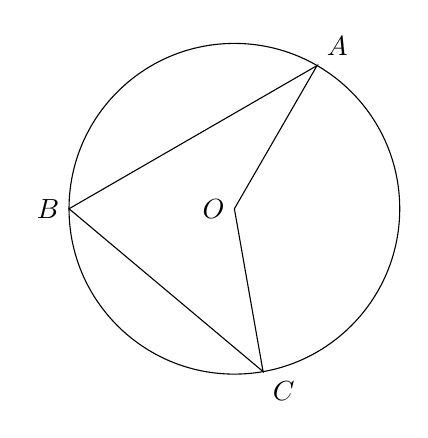
\begin{tikzpicture}[scale=2.1]
  \coordinate (O) at (0,0); % Center of the circle
  \draw (O) circle (1); % Unit circle
  
  % Points on the circle
  \coordinate (A) at (60:1); % Point A at angle 60 degrees
  \coordinate (B) at (180:1); % Point B at angle 180 degrees
  \coordinate (C) at (280:1); % Point C at angle 300 degrees
  
  % Dart OABC
  \draw (O) -- (A) -- (B) -- (C) -- cycle;
  
  % Labels for points A, B, C
  \node at (A) [above right] {$A$};
  \node at (B) [left] {$B$};
  \node at (C) [below right] {$C$};
  
  % Center label O
  \node at (O) [left] {$O$};
\end{tikzpicture}

\end{center}
\end{minipage}

\question[0] \textbf{Bonus.} Find the length $\overline{AC}$ in the dart above, to 2 decimal places.

\fillwithdottedlines{\stretch{1}}

\end{questions}

\begin{tcolorbox}

\textbf{Name of the marker:}

\begin{center}
\gradetable[h][questions]
\end{center}

\end{tcolorbox}

\end{document}